\section{Using the commandline / terminal}
% ----------------------------------
\begin{frame}[fragile,allowframebreaks]{Terminal/Commandline basics}
\footnotesize
\metroset{block=fill}

\begin{columns}
\column{0.55\textwidth}

\begin{block}{Navigating in the terminal}
\begin{enumerate}
    \item search for ``terminal''/``cmd''. The prompt will tell you your current location in the file system, e.g. \texttt{c:} in Windows 
\item To show contents of current directory:
\begin{itemize}\scriptsize
    \item \texttt{dir} (Windows)
    \item \texttt{ls} (Linux/Unix)
\end{itemize}
\item change directory = \texttt{cd directoryname} or use absolute path:
\begin{itemize}\scriptsize
    \item \texttt{cd my/path} (Windows)
    \item \verb|cd my\path| (Unix)
\end{itemize} 
\item back one directory: \texttt{cd ..}
\item open Sqlite3 (you have to be in the folder where \texttt{sqlite3.exe} lies or is accessible from): 
\begin{verbatim}
    sqlite3
\end{verbatim}
\end{enumerate}
\end{block}

\column{0.5\textwidth}

\begin{alertblock}{Most important commands for navigating the filesystem in the terminal}
\begin{description}
    \item[dir/ls] show directory contents:
    \begin{itemize}\footnotesize
    \item \texttt{dir} (Windows)
    \item \texttt{ls} (Linux/Unix)\end{itemize}
    \item[cd path] change directory (\texttt{cd directoryname} or absolute path):
    \begin{itemize}\footnotesize
    \item \texttt{cd my/path} (Windows)
    \item \verb|cd my\path| (Unix)
    \end{itemize} 
    \item[cd ..] back one directory
\end{description}
\end{alertblock}
\end{columns}

%---

\framebreak

\begin{columns}
\column{0.61\textwidth}

E.g.. Linux / Unix / \textasciitilde Mac
\begin{shell-sessioncode}
sary@laptop:~$ cd Desktop
sary@laptop:~/Desktop$ ls
 studis.db 
sary@laptop:~/Desktop$ sqlite3 studis.db
SQLite version 3.32.3 2020-06-18 14:00:33
sqlite> .quit
sary@laptop:~/Desktop$ sqlite3 
SQLite version 3.32.3 2020-06-18 14:00:33
Enter ".help" for usage hints.
Connected to a transient in-memory database.
Use ".open FILENAME" to reopen on a
persistent database.
sqlite> .open studis.db
sqlite> .tables
fachgebiet
\end{shell-sessioncode}

If no success: install first or\dots 
\begin{shell-sessioncode}
sary@laptop:~/Desktop$ which sqlite3
/home/oem/anaconda3/bin/sqlite3
sary@laptop:~/Desktop$ sqlite3 -version
3.32.3 2020-06-18 14:00:33 ...
\end{shell-sessioncode}

\column{0.45\textwidth}

E.g. Windows

\begin{block}{Search: `Terminal/cmd'}
Show contents of currenct directory
\begin{shell-sessioncode}
C:\> dir
 Datenträger in Laufwerk C: 
 ist System ....
 Verzeichnis von C:\Users 
 18.01.2022 14:22 <DIR> sarah
 22.03.2022 10:07 <DIR> test
\end{shell-sessioncode}

Change directory
\begin{shell-sessioncode}
C:\> cd Users\sarah
\end{shell-sessioncode}

Change harddrive
\begin{shell-sessioncode}
C:\Users\sarah> Z:
\end{shell-sessioncode}
\end{block}
\end{columns}
\end{frame}

\section{Open SQLite3 in the terminal}
% ----------------------------------
\begin{frame}[fragile,allowframebreaks]{Sqlite3 Setup}
\footnotesize
\metroset{block=fill}

\begin{block}{How to get (to) Sqlite3?}
\begin{itemize}
    \item Installation: \protect\url{https://www.tutorialspoint.com/sqlite/sqlite_installation.htm}
    \item If Windows: \protect\url{https://www.sqlite.org/download.html} > Precompiled Binaries for Windows > \texttt{sqlite-tools-win32-x86-3360000.zip}
    \item Unzip file, in case of Windows: put \texttt{sqlite3.exe} in the same directory as \texttt{studis.db} \& \texttt{ urlaub.db } 
    \begin{itemize}
        \item best not a complicated long file path 
        \item best no spaces/special characters in the filenames or paths
    \end{itemize}
    \item \texttt{Alternatively:} Just use the \texttt{.zip} from Moodle, unzip (!), put all data in one same directory (\texttt{sqlite.exe} \& \texttt{.db} files have to be in the same directory!). 
\end{itemize}
\end{block}

\framebreak

Example ouput from a fromer student under Windows: 

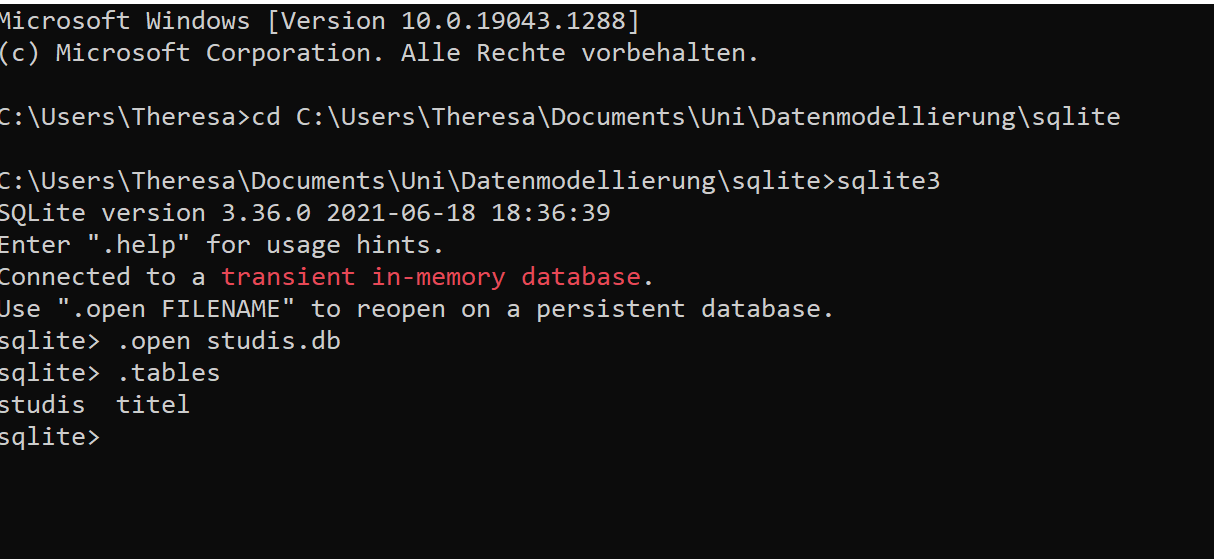
\includegraphics[width=\textwidth]{img/how_to_open_file_in_windows_sqlite3.png}

\framebreak
%---

In Sqlite3 (you can tell you're in because it says \texttt{sqlite3>} in front):
\begin{sqlcode}
.open studis.db
.tables
SELECT * FROM studis;
\end{sqlcode}
Don't forget the semicolon at the end!

Maybe before that run:
\begin{sqlcode}
.mode columns
.headers on
\end{sqlcode}

\framebreak

\begin{block}{Troubleshooting}
\begin{itemize}\small
    \item After \texttt{.open studis.db} ideally there is no output $\to$ check using \texttt{.tables} if there's any database content yet. 
    \item If there's nothing, maybe try \texttt{which sqlite3} in Mac (might not open the file you wanted but another path $\to$ navigate to correct location). 
    \item Upon clicking \texttt{sqlite3.exe } this should work under Windows but your database \texttt{studis.db} file really has to be in the same directory!
    \item Does \texttt{studis.db} seem empty? Did you open it with DB-Browser previously? This can sometimes delete the contents $\to$ re-download from Moodle and open directly via the terminal. 
\end{itemize}
\end{block}

\framebreak

\begin{block}{Potential problems}
\begin{enumerate}\small
    \item There is no data where you currently are, meaning that SQLite3 will not find anything. 
    \item You are where the data are but from there, SQLite3 cannot be accessed (maybe set environment variable or put \texttt{sqlite3.exe} into the folder). 
\end{enumerate}
\end{block}

\end{frame}

% ----------------------------------
\begin{frame}[fragile,allowframebreaks]{First SQL exercise}
\footnotesize
\metroset{block=fill}


Try these commands for the first exercise:

\begin{enumerate}
    \item First open a \texttt{.db} file as indicated above:
\begin{sqlcode}
.tables -- 2 should appear
.headers on -- maybe improve the visuals
.mode column
\end{sqlcode}

\item We create a table called \texttt{disciplines/fachgebiete}:
\begin{sqlcode}
CREATE TABLE fachgebiete (id INT, name TEXT);
.tables
\end{sqlcode}
\item $\to$ a new table should appear but it's still empty when you try the following command:
\begin{sqlcode}
SELECT * FROM fachgebiete;
\end{sqlcode}
\item  Add a new column \texttt{fachgebiet\_id}  to \texttt{studis}:  
\begin{sqlcode}
ALTER TABLE studis 
ADD COLUMN fachgebiet_id INT;
\end{sqlcode}
\item Then add both values:
\begin{sqlcode}
INSERT INTO studis (name, fachgebiet_id) 
VALUES ("Max Mara", 1);
\end{sqlcode}
or update if this row already exists (all get overwritten with value 1): 
\begin{sqlcode}
UPDATE studis SET fachgebiet_id=1;
\end{sqlcode}

\item You can put conditions $\to$ e.g.. update \texttt{studis} with \texttt{id=1} \& \texttt{id=4}, then set their discipline id to \texttt{1}:
\begin{sqlcode}
UPDATE studis SET fachgebiet_id=1 
WHERE (id = 1) AND (id = 4);
\end{sqlcode}
\item Using \texttt{.schema} I can check the setup of a table again. And save like so:
\begin{sqlcode}
.save studis_neu.db
\end{sqlcode}
\end{enumerate}

%------------------------

\begin{columns}
\column{0.5\textwidth}
$\to$ Pressing the arrow-up key gives you your last commands so you don't need to retype them each time.

$\to$ Youtube-Video to go along with the SQL basics exercise: \protect\url{https://www.youtube.com/watch?v=TpY1D13J7So} 

\column{0.43\textwidth}
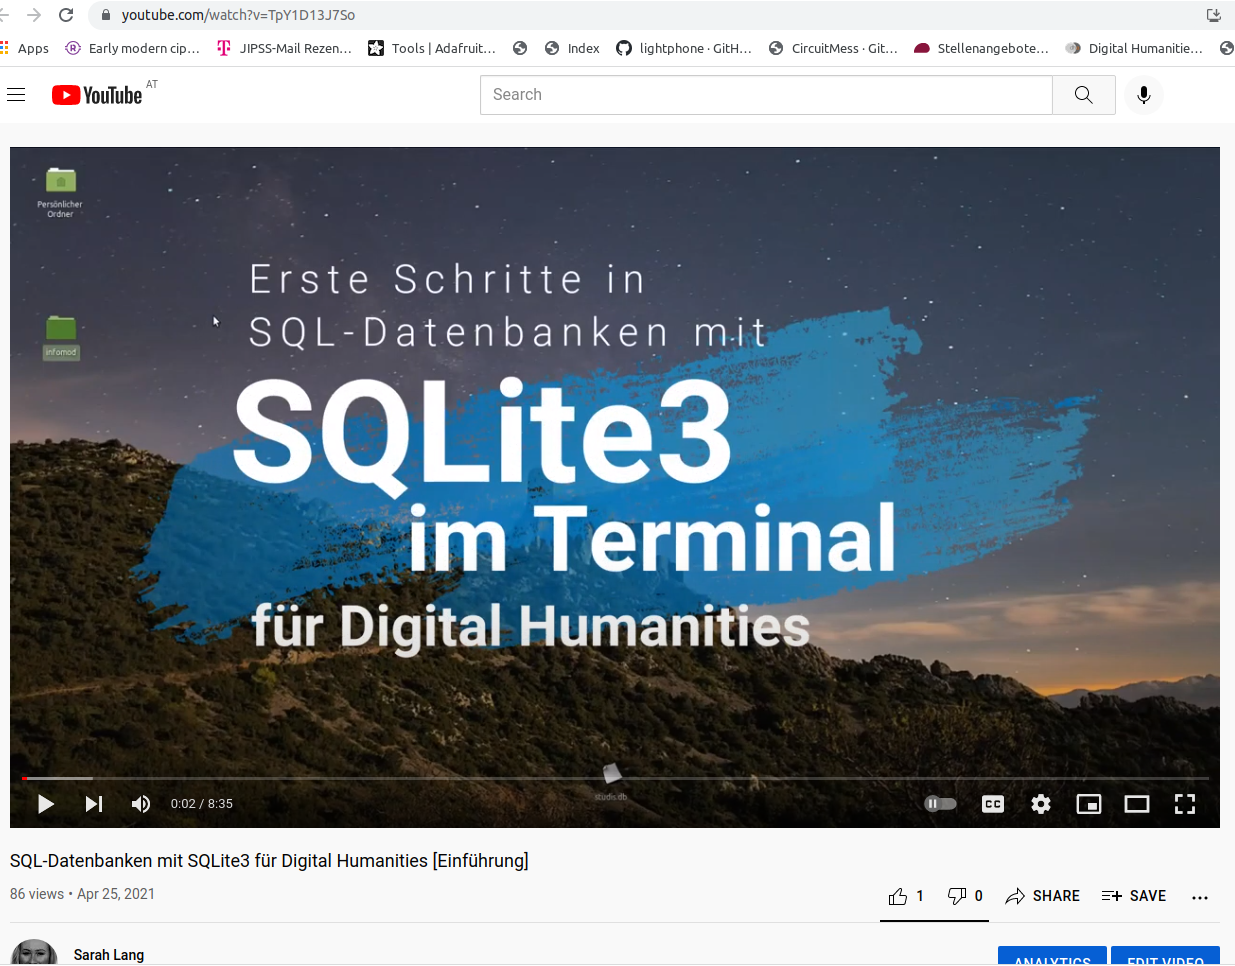
\includegraphics[width=\textwidth]{img/sql-basics-video-youtube.png}

\end{columns}

\end{frame}

%--------------------------------------------------
\begin{frame}[fragile]{CSV Import}
\small \metroset{block=fill}
    Usually you can download/export spreadsheets as \texttt{.csv}.
    You should be able to import this in SQLite3 as a table using the following command (example \texttt{city.csv} imported as a newly created table called \texttt{cities}).
\begin{sqlcode}
sqlite> .import c:/sqlite/city.csv cities
\end{sqlcode}

\begin{columns}
\column{0.48\textwidth}
Create table
\begin{sqlcode}
CREATE TABLE cities (
  name TEXT NOT NULL,
  population INTEGER NOT NULL 
);
\end{sqlcode}

\column{0.48\textwidth}
CSV Import
\begin{sqlcode}
.mode csv
.import c:/sqlite/city.csv cities
\end{sqlcode}
\end{columns}

\textbf{Tutorial:} \protect\url{https://www.sqlitetutorial.net/sqlite-import-csv/}


\end{frame}
%--------------------------------------------------

\begin{frame}[fragile]{Saving your database}
\metroset{block=fill}

    
\begin{shell-sessioncode}
oem@sary-ThinkPad-X270:~$ sqlite3
SQLite version 3.32.3 2020-06-18 14:00:33
Enter ".help" for usage hints.
Connected to a transient in-memory database.
Use ".open FILENAME" to reopen on a persistent database.
sqlite> 
\end{shell-sessioncode}


\begin{block}{Save results}
How to use \texttt{.dump} / \texttt{.save} and \texttt{.open} again
\begin{itemize}\footnotesize
    \item \protect\url{https://www.sqlitetutorial.net/sqlite-dump/}
    \item \protect\url{https://sqlite.org/cli.html}
\end{itemize}
\end{block}

\begin{sqlcode}
.save example.db
\end{sqlcode}
\protect\url{https://sqlite.org/cli.html} $\to$ under \texttt{.save}

% ----------------------------------

\end{frame}